\section{Molecules in space}
\label{sec:intro:ions_in_space}

\epigraph{Somewhere, something incredible is waiting to be known}{Carl Sagan}
Sir Arthur Stanley Eddington's Bakerian Lecture on \enquote{\emph{Diffuse matter in interstellar space}} \cite{eddington_bakerian_1926} of 1926 may be a natural starting point for the discussion of molecules in the interstellar medium. The sharp calcium spectral line observed by \citet{hartmann_investigations_1904} in 1904 and the subsequent discovery of D-lines of sodium (\citet{heger_occurrence_1919} in 1919) and H and K lines of calcium (\citet{plaskett_h_1923} in 1923) were the premises of Eddington's discussion. These lines were not arising from absorption in either the stellar atmosphere or Earth's atmosphere. Since they were also unaffected by stellar motion, they were known as \emph{fixed} or \emph{stationary} lines. These lines were assumed to originate from interstellar space. Eddington pointed out in his lecture that \enquote{...it is difficult to admit the existence of molecules in interstellar space because when once a molecule becomes dissociated, there seems no chance of the atoms joining up again}. 

\subsection{Optical observation}
\label{subsec:intro:optical}

In the early 1930s, \citet{merrill_unidentified_1934} identified several interstellar lines (much wider than interstellar atomic lines) of unknown origin. \citet{russell_analysis_1935} conjectured that the origin of these lines was molecular rather than atomic. \citet{merrill_stationary_1936} noted that \enquote{the chemical identification of these lines had not been made yet}, and remarkably, the chemical identity is unknown even today for these \emph{diffuse interstellar bands} (DIBs). An exception is C$_{60}^+$ which is the only species identified as the carrier of two DIBs by \citet{campbell_laboratory_2015} only recently in 2015, based on laboratory action spectroscopic methods similar to the ones described in this thesis. However, hundreds of DIBs remain to be identified. Hence, it remains the oldest unsolved problem in astronomical spectroscopy. Nevertheless, it became clear that the interstellar absorption lines could not all be due to neutral or ionized atoms.

Later, in the late 1930s, Adams, Dunham and McKellar established the presence of CH, CN and CH$^+$ molecular species in the interstellar medium based on four sharp absorption lines seen in the optical spectra of several distant stars using Mount Wilson Observatory (\citet{dunham_jr_interstellar_1937} 1937, \citet{adams_quoted_1937} 1937, \citet{mckellar_evidence_1940, mckellar_wave_1940} 1940) and laboratory data (\citet{jenkins_mass_1938, douglas_note_1941, douglas_band_1942}). Three interstellar molecules were identified in four years, one of which was a positively charged ion. Detailed quantitative studies by \citet{bates_density_1951} in 1951, and its extension by \citet{solomon_formation_1972} in 1972 and \citet{herbst_formation_1973} in 1973, to understand the formation of these interstellar molecular species showed the crucial role of ion-molecule reactions.

\subsection{Radio observation}
\label{subsec:intro:radio}

The hydroxyl radical (OH) molecule has a ground state of $^2\Pi$, resembling CH. However, its optical resonance lines lie in the 3060 $\mathring{\text{A}}$ region, close to the atmosphere's edge of transmission. Due to interference from our own atmosphere's ozone absorption bands, it is challenging to observe these lines. \citet{weinreb_radio_1963} \citeyear{weinreb_radio_1963} observed the first lines of OH near radio frequency 1665 MHz, which represents a transition between the $\Lambda$ doublet components of the lowest rotational level $J=3/2$ of $^2\Pi_{3/2}$ (hyperfine structure). The radio detection of OH inspired many radio astronomers to consider the possibilities of detecting polyatomic molecule lines in the radio frequency range. \citet{cheung_detection_1968} succeeded in 1968 with NH$_3$ and shortly after with H$_2$O \cite{cheung_detection_1969}, both in emission. \citet{snyder_microwave_1969} soon discovered formaldehyde (H$_2$CO) in absorption; numerous new compounds have been discovered annually, a trend that has continued at a nearly linear rate ever since \cite{mcguire_2021_2021}.

\subsection{Infrared observation}
\label{subsec:intro:IR}

\citet{gillett_8_1973} using ground observations, discovered three distinct emission bands in the 8 - 13 $\mu$m spectra of two planetary nebulae (NGC 7027 and 6572), ushering in a new era in astrochemistry in the early 1970s. \citet{merrill_2_1975} reported the detection of a broad emission band in NGC 7027 two years later. Airborne observations also became feasible during that period for the first time. This allowed the Kuiper Airborne Observatory (KAO) to find two new, unreachable from the ground, powerful emission bands in NGC 7027 and an external galaxy (M82) \cite{russell_4_1977, willner_2_1977}. These characteristics were subsequently discovered to be widespread throughout the cosmos and closely related, forming the PAH family (PAH=Polycyclic Aromatic Hydrocarbons). Although the precise nature of the carriers of these features is still unknown, they have been collectively referred to as unidentified infrared emission (UIE) features. However, the hypothesis that PAH molecules serve as carriers has received significant support \cite{leger_identification_1984, allamandola_polycyclic_1985}. The PAHs in ISM are postulated to be 
assembled by smaller molecules, and smaller molecular ions plays an important role as an intermediate 
as well the main driving force of interstellar chemistry \cite{smith_ion_1992,herbst_dense_1988,CGP2015}.

\begin{figure}[!htb]
    \centering
    \includegraphics[scale=0.3]{figures/intro/JWST.jpg}
    \caption{James Webb Space Telescope - An infrared-optimized astronomical observatory (Credit: NASA)}
    \label{fig:JWST}
\end{figure}

Recently, the James Webb Space Telescope (JWST), as shown in Figure \ref{fig:JWST} was launched in late 2021. It is an infrared-optimized astronomical observatory which will operate in near- ($0.6 - 5$ $\mu$m) and mid- ($5 - 28$ $\mu$m) infrared regions \footnote{\url{https://www.jwst.nasa.gov/content/observatory/instruments/index.html}} to address a range of astrophysical and cosmological questions, including the role of PAHs.

\subsection{Current status}
Astronomers are now aware of many additional diatomic and polyatomic molecules in the ISM. Furthermore, a large number of unknown species await their identification, such as the UIE and DIBs. As of late May 2022, about 270 molecules have been detected in the ISM or circumstellar shells (CDMS database\footnote{\url{https://cdms.astro.uni-koeln.de/classic/molecules}}), and $\sim 12 \%$ of them are cationic species \cite{mcguire_2021_2021} see Figure \ref{fig:ISM_molecules}. Interstellar molecules can be identified through their electronic (optical), vibrational (infrared), and rotational (radio) spectra as shown in Sections \ref{subsec:intro:optical} through \ref{subsec:intro:IR}. However, most ($\sim$ 80 \%) of interstellar species are identified via their rotational transition \cite{mcguire_2021_2021} because of their low excitation temperature and distinct spectroscopic  fingerprint. In conclusion, one can say that laboratory spectroscopic data are indeed vital in identifying these molecular species in space. This is difficult for highly reactive molecular ions, but their laboratory characterization and subsequent astronomical detection are important to understand the ion-molecule chemistry of the ISM. Therefore, in the next section, a brief introduction to spectroscopy followed by a detailed review of spectroscopic methods especially for studying molecular ions are presented.

\begin{figure}[!htb]
    \centering
    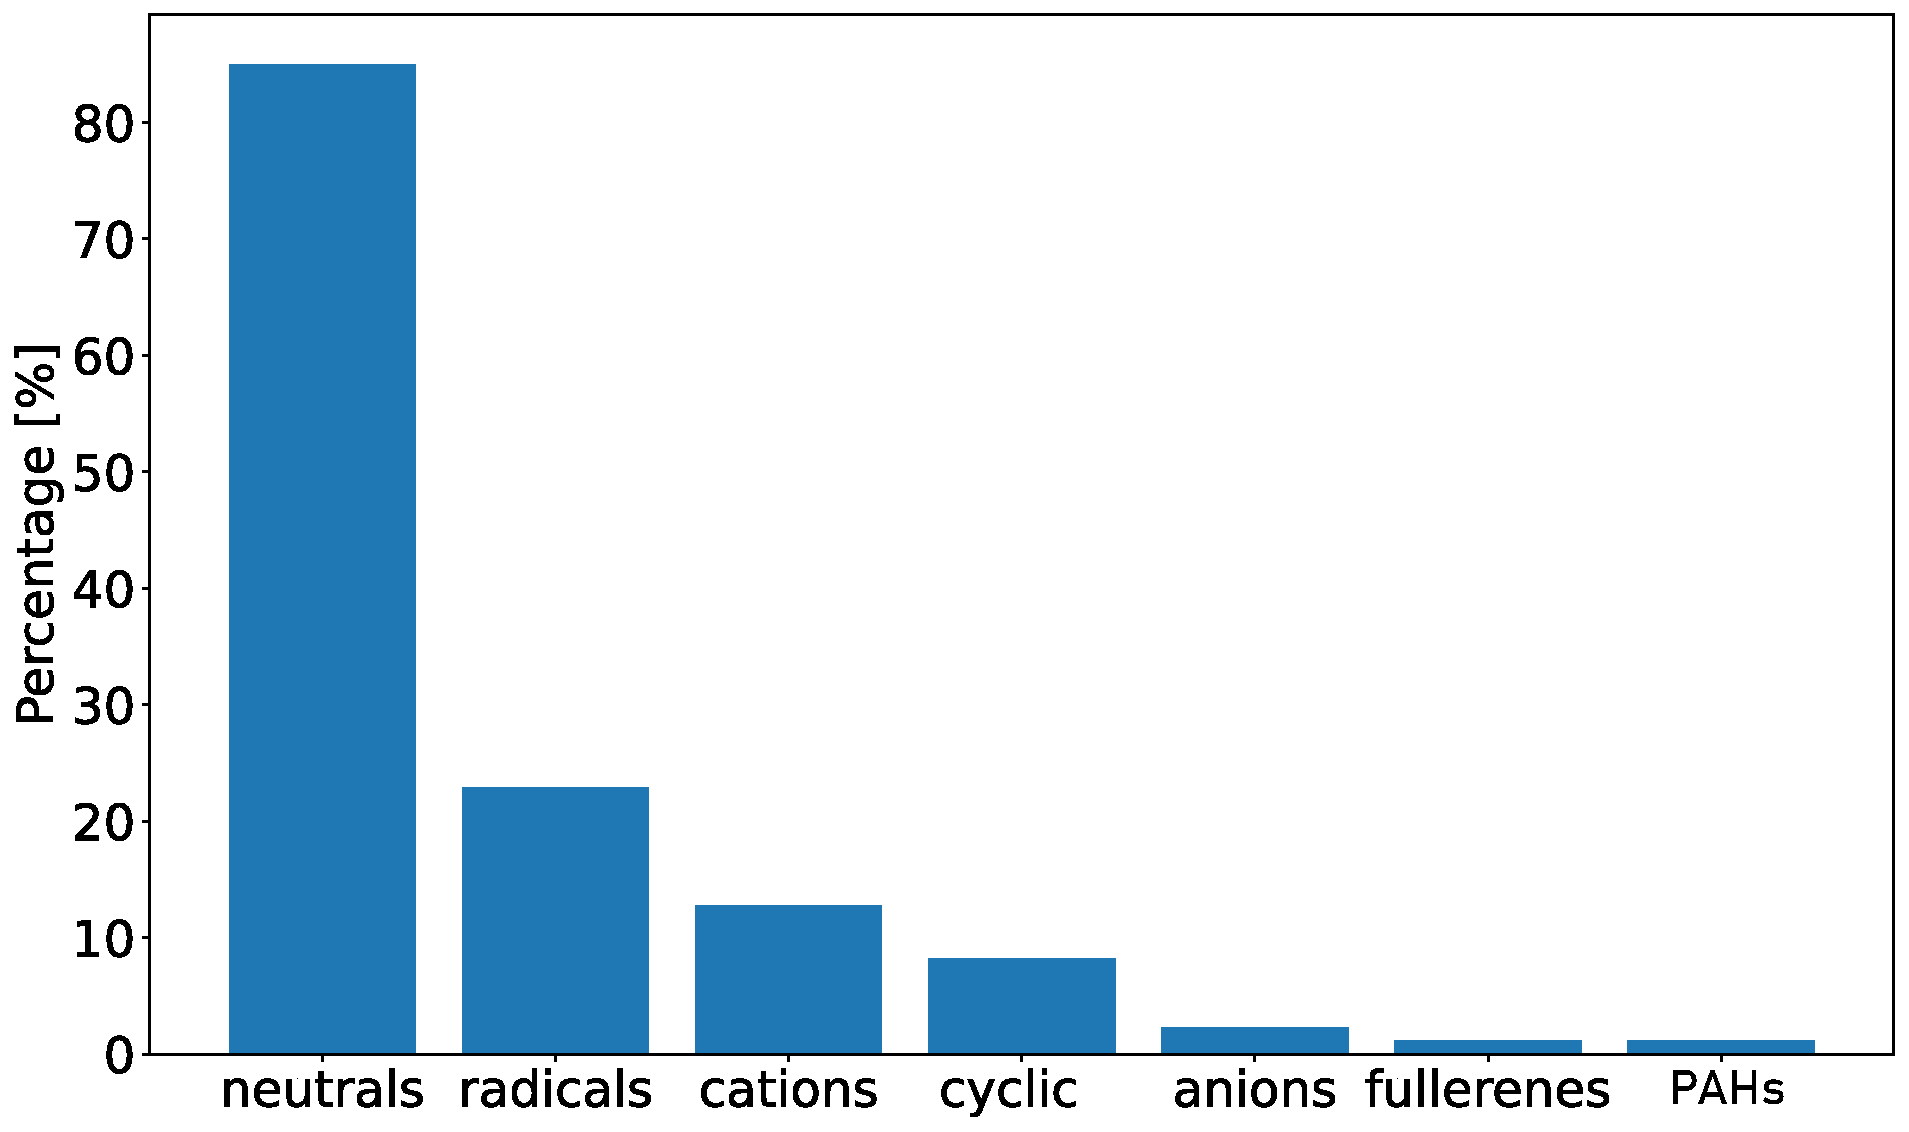
\includegraphics[width=0.75\textwidth]{figures/intro/known_molecules_in_space.pdf}
    \caption{Percentage of different classes of  known interstellar molecules. Many molecules fall into more than one of these categories \emph{e.g.} most radical species have a net neutral charge. Data is computed using \emph{astromol - A Database of Molecules Detected in Space} python library \cite{mcguire_astromol_2021}}
    \label{fig:ISM_molecules}
\end{figure}
